\documentclass[12pt, a4paper]{article}

% Packages
\usepackage[utf8]{inputenc}
\usepackage[T1]{fontenc}
\usepackage[french]{babel}
\usepackage{geometry}
\usepackage{xcolor}
\usepackage{tabularx}
\usepackage{booktabs}
\usepackage{hyperref}
\usepackage{titlesec}
\usepackage{enumitem}
\usepackage{fancyhdr}
\usepackage{tcolorbox}
\usepackage{graphicx}
\usepackage{array}
\usepackage{multirow}
\usepackage{float}

% Configuration des marges
\geometry{left=2.5cm, right=2.5cm, top=2.5cm, bottom=2.5cm}

% Couleurs du rapport
\definecolor{mlblue}{RGB}{0, 120, 212}
\definecolor{rfgreen}{RGB}{16, 124, 16}
\definecolor{successgreen}{RGB}{16, 124, 16}
\definecolor{warningorange}{RGB}{255, 140, 0}
\definecolor{riskred}{RGB}{226, 75, 74}

% Configuration des liens
\hypersetup{
    colorlinks=true,
    linkcolor=mlblue,
    urlcolor=mlblue,
    citecolor=mlblue,
    hypertexnames=false
}

% Configuration des sections
\titleformat{\section}{\Large\bfseries\color{mlblue}}{\thesection}{1em}{}
\titleformat{\subsection}{\large\bfseries\color{rfgreen}}{\thesubsection}{1em}{}

% En-tête et pied de page
\pagestyle{fancy}
\fancyhf{}
\fancyhead[L]{Projet ML : Prédiction Customer Churn}
\fancyhead[R]{4IASD}
\fancyfoot[C]{\thepage}
\setlength{\headheight}{15pt}

% Environnements
\newtcolorbox{infobox}{
    colback=mlblue!5,
    colframe=mlblue,
    title=Information,
    sharp corners,
    boxrule=0.5mm
}

\newtcolorbox{warningbox}{
    colback=warningorange!5,
    colframe=warningorange,
    title=Point de vigilance,
    sharp corners,
    boxrule=0.5mm
}

\newtcolorbox{datasetbox}{
    colback=rfgreen!5,
    colframe=rfgreen,
    title=Dataset,
    sharp corners,
    boxrule=0.5mm
}

\newcommand{\filepath}[1]{\texttt{\detokenize{#1}}}
\newcommand{\TitreProjet}{Développement d'un Système de Prédiction du Churn Client}
\newcommand{\SousTitreProjet}{Machine Learning avec XGBoost, CatBoost et Streamlit}
\newcommand{\EtudiantUn}{Oumaima \textsc{Channani}}
\newcommand{\EtudiantDeux}{Othmane \textsc{Amine}}
\newcommand{\FiliereProjet}{4IASD}
\newcommand{\EncadrantProjet}{Prof. Oussama Elgerari}
\newcommand{\AnneeUniversitaire}{2025--2026}
\newcommand{\ImageOuCadre}[4]{%
  \IfFileExists{#1}{%
    \includegraphics[width=#2,height=#3,keepaspectratio]{#1}%
  }{%
    \fbox{%
      \begin{minipage}[c][#3][c]{#2}
        \centering\small\color{gray!70}#4
      \end{minipage}%
    }%
  }%
}

\begin{document}

%==============================================================================
% Page de titre
%==============================================================================
\begin{titlepage}
    \newgeometry{top=1.15cm,bottom=1.05cm,left=1.65cm,right=1.65cm}
    \thispagestyle{empty}
    \centering

    \begin{minipage}[c]{0.44\textwidth}
        \centering
        \ImageOuCadre{logo_emsi.png}{0.9\linewidth}{2.5cm}{Logo EMSI}
    \end{minipage}
    \hfill
    \begin{minipage}[c]{0.44\textwidth}
        \centering
        \ImageOuCadre{logo_ecole2.jpeg}{0.9\linewidth}{2.5cm}{Logo établissement}
    \end{minipage}

    \vspace{3cm}
    {\large\bfseries Filière Science de Données et Intelligence Artificielle\par}

    \vspace{1.5cm}
    {\Large\bfseries Rapport technique de projet de fin d'année\par}

    \vspace{2cm}
    \setlength{\fboxrule}{1.1pt}
    \setlength{\fboxsep}{13pt}
    \fbox{%
      \begin{minipage}{0.9\textwidth}
        \centering
        {\LARGE\bfseries\color{mlblue}\TitreProjet\par}
        \vspace{0.45cm}
        {\large\bfseries\color{rfgreen}\SousTitreProjet\par}
      \end{minipage}%
    }

    \vspace{2cm}
    {\large Présenté le \today\par}

    \vspace{3cm}
    \begin{minipage}[t]{0.50\textwidth}
      \raggedright
      {\large\bfseries Réalisé par :\par}
      \vspace{0.35cm}
      \EtudiantUn \quad(\FiliereProjet)\par
      \vspace{0.22cm}
      \EtudiantDeux \quad(\FiliereProjet)\par
    \end{minipage}
    \hfill
    \begin{minipage}[t]{0.38\textwidth}
      \raggedright
      {\large\bfseries Encadré par :\par}
      \vspace{0.35cm}
      -- \EncadrantProjet\par
    \end{minipage}

    \vfill
    {\large\bfseries Année universitaire : \AnneeUniversitaire\par}
    \vspace{0.35cm}

    \restoregeometry
\end{titlepage}

%==============================================================================
% Résumé
%==============================================================================
\newpage
\thispagestyle{plain}
\begin{center}
    {\LARGE\bfseries\color{mlblue}Résumé\par}
\end{center}
\vspace{0.8cm}

La fidélisation des clients constitue un enjeu stratégique majeur pour les
opérateurs de télécommunications, car l'acquisition d'un nouvel abonné est
généralement plus coûteuse que la conservation d'un client existant. Ce projet
a pour objectif de concevoir et de mettre en œuvre un système intelligent
capable d'anticiper le churn client, d'expliquer les facteurs associés au risque
de départ et de proposer des actions de fidélisation adaptées aux profils
identifiés.

L'étude s'appuie sur un dataset télécom composé de 7\,043 clients et de 21
variables décrivant notamment leur profil, leur ancienneté, leur contrat, les
services souscrits, leur méthode de paiement et leurs charges. Une chaîne de
prétraitement reproductible a été développée afin de nettoyer les données,
traiter les valeurs manquantes, convertir les variables numériques et encoder
les attributs catégoriels. La séparation stratifiée en jeux d'entraînement
(80\,\%) et de test (20\,\%) est effectuée avant l'ajustement du préprocesseur,
ce qui limite les risques de fuite d'information et garantit une évaluation
plus rigoureuse.

Trois modèles de classification ont été entraînés et comparés : XGBoost,
CatBoost et la régression logistique. Leur performance a été mesurée avec
l'Accuracy, la Precision, le Recall, le F1-score, le ROC-AUC et les matrices de
confusion. Parmi les modèles de base, CatBoost obtient les meilleurs résultats
globaux avec une Accuracy de 0,756, un Recall de 0,789, un F1-score de 0,632 et
un ROC-AUC de 0,842. Une optimisation par validation croisée améliore ensuite
le ROC-AUC test de XGBoost jusqu'à 0,847 et confirme la proximité des
performances de XGBoost et CatBoost.

L'analyse exploratoire et l'étude de l'importance des variables montrent que le
contrat mensuel, la faible ancienneté, les charges élevées, l'utilisation de la
fibre optique, l'absence de support technique et le paiement par chèque
électronique sont fortement associés au risque de churn. Ces résultats sont
transformés en segments de risque faible, moyen ou élevé, puis en
recommandations métier personnalisées, telles qu'un appel prioritaire, une
remise ciblée ou une proposition de contrat annuel.

Enfin, les modèles et le préprocesseur sont intégrés dans une application et un
dashboard Streamlit. Ces interfaces permettent respectivement d'obtenir une
prédiction individuelle avec sa probabilité et d'analyser les tendances
globales du portefeuille client. La solution proposée fournit ainsi un outil
d'aide à la décision complet, interprétable et directement exploitable pour
orienter les campagnes de fidélisation.\\\\


\noindent\textbf{Mots-clés :} churn client, télécommunications, machine
learning, XGBoost, CatBoost, classification, feature importance, fidélisation,
Streamlit.

%==============================================================================
% Abstract
%==============================================================================
\newpage
\thispagestyle{plain}
\begin{center}
    {\LARGE\bfseries\color{mlblue}Abstract\par}
\end{center}
\vspace{0.8cm}

Customer retention is a major strategic concern for telecommunications
companies, as acquiring a new subscriber is generally more expensive than
retaining an existing customer. This project aims to design and implement an
intelligent system capable of anticipating customer churn, explaining the main
factors associated with departure risk, and recommending suitable retention
actions for the identified customer profiles.

The study relies on a telecommunications dataset containing 7,043 customers and
21 variables describing customer profiles, tenure, contracts, subscribed
services, payment methods, and charges. A reproducible preprocessing workflow
was developed to clean the data, handle missing values, convert numerical
attributes, and encode categorical features. A stratified 80/20 train-test
split is performed before fitting the preprocessing components, reducing data
leakage and ensuring a rigorous evaluation process.

Three classification models were trained and compared: XGBoost, CatBoost, and
Logistic Regression. Their performance was assessed using Accuracy, Precision,
Recall, F1-score, ROC-AUC, and confusion matrices. Among the baseline models,
CatBoost achieved the best overall results, with an Accuracy of 0.756, a Recall
of 0.789, an F1-score of 0.632, and a ROC-AUC of 0.842. Cross-validation-based
hyperparameter optimization further increased XGBoost's test ROC-AUC to 0.847
and confirmed the close predictive performance of XGBoost and CatBoost.

Exploratory analysis and feature importance results indicate that month-to-month
contracts, short tenure, high charges, fiber-optic Internet service, lack of
technical support, and electronic check payments are strongly associated with
churn risk. The predicted probabilities are converted into low, medium, and
high-risk segments and linked to personalized business recommendations,
including priority calls, targeted discounts, and annual contract offers.

Finally, the trained models and preprocessing pipeline are integrated into a
Streamlit prediction application and an analytical dashboard. These interfaces
support both individual churn prediction and portfolio-level analysis. The
resulting solution provides a complete, interpretable, and operational
decision-support tool for improving customer retention strategies.\\\\


\noindent\textbf{Keywords:} customer churn, telecommunications, machine
learning, XGBoost, CatBoost, classification, feature importance, customer
retention, Streamlit.

\newpage
\tableofcontents
\newpage

\phantomsection
\addcontentsline{toc}{section}{Liste des figures}
\listoffigures
\newpage

\phantomsection
\addcontentsline{toc}{section}{Liste des tableaux}
\listoftables
\newpage

%==============================================================================
\section*{Introduction générale}
\addcontentsline{toc}{section}{Introduction générale}

La transformation numérique des entreprises a considérablement augmenté la
quantité de données disponibles sur les comportements et les usages des
clients. Dans le secteur des télécommunications, chaque interaction laisse des
traces exploitables : durée de la relation, services activés, type de contrat,
mode de paiement, facturation et historique des charges. L'analyse de ces
informations permet de mieux comprendre les attentes des abonnés et
d'anticiper les situations susceptibles de conduire à une résiliation.

Le churn client représente la perte d'un abonné au profit d'un concurrent ou
à la suite d'une interruption volontaire du service. Son impact dépasse la
simple diminution du nombre de clients. Il peut entraîner une baisse du revenu
récurrent, une augmentation des dépenses commerciales et une dégradation de la
valeur vie client. Une stratégie uniquement réactive intervient souvent trop
tard. À l'inverse, un système prédictif peut hiérarchiser les clients selon
leur niveau de risque et permettre aux équipes métier d'agir avant la
résiliation.

La problématique étudiée dans ce rapport est donc la suivante :
\begin{quote}
\textit{Comment construire un système de machine learning fiable,
interprétable et exploitable permettant de prédire le churn client et de
transformer les résultats du modèle en actions de fidélisation concrètes ?}
\end{quote}

Pour répondre à cette problématique, le projet met en place une démarche
complète. Elle débute par l'analyse et la préparation d'un dataset télécom,
puis compare plusieurs modèles de classification supervisée. Les performances
sont évaluées selon plusieurs métriques afin de ne pas limiter l'analyse à
l'Accuracy, particulièrement insuffisante lorsque les classes sont
déséquilibrées. L'interprétation des variables influentes complète cette
évaluation et permet de relier les résultats statistiques à des décisions
métier.

Le rapport est organisé en trois chapitres principaux. Le premier présente les
données, leur qualité, le prétraitement et les enseignements de l'analyse
exploratoire. Le deuxième détaille le protocole expérimental, les modèles,
leurs métriques et l'optimisation des hyperparamètres. Le troisième traite de
l'interprétation, de la segmentation du risque, des recommandations de
fidélisation et de l'intégration dans Streamlit. Une conclusion générale
synthétise enfin les apports, les limites et les perspectives du projet.

\newpage

%==============================================================================
\section{Informations Générales}

\subsection{Contexte et problématique}

Le churn client désigne la décision d'un abonné de quitter un service. Dans le
secteur des télécommunications, cette situation entraîne une perte de revenu et
un coût d'acquisition supplémentaire pour remplacer le client. L'objectif du
projet est de détecter les clients susceptibles de résilier leur abonnement afin
de déclencher une action de fidélisation adaptée.

\begin{infobox}
Le système développé couvre toute la chaîne de valeur : préparation des données,
analyse exploratoire, entraînement et comparaison des modèles, interprétation
des prédictions, recommandations métier et mise à disposition dans une
application Streamlit.
\end{infobox}

\subsection{Objectifs}

Les objectifs techniques et métier du projet sont les suivants :
\begin{itemize}[leftmargin=*]
    \item construire un pipeline reproductible de nettoyage, d'imputation et
    d'encodage des données ;
    \item entraîner XGBoost et CatBoost, puis les comparer à une régression
    logistique de référence ;
    \item évaluer les modèles avec Accuracy, Precision, Recall, F1-score,
    ROC-AUC et matrices de confusion ;
    \item identifier les variables qui influencent le plus le churn ;
    \item fournir une probabilité de churn et une recommandation de
    fidélisation dans une interface Streamlit.
\end{itemize}

\subsection{Architecture de la solution}

\begin{center}
\begin{tcolorbox}[colback=mlblue!3,colframe=mlblue,width=0.92\textwidth]
\centering
\textbf{Dataset CSV}\\
$\downarrow$\\
\textbf{Nettoyage et séparation Train/Test}\\
$\downarrow$\\
\textbf{Imputation et encodage ajustés sur Train}\\
$\downarrow$\\
\textbf{Entraînement XGBoost, CatBoost et Régression Logistique}\\
$\downarrow$\\
\textbf{Évaluation, feature importance et sauvegarde des modèles}\\
$\downarrow$\\
\textbf{Application de prédiction et dashboard Streamlit}
\end{tcolorbox}
\end{center}

L'organisation modulaire sépare le prétraitement
(\filepath{src/preprocessing.py}), l'entraînement
(\filepath{src/training.py}), la prédiction
(\filepath{src/prediction.py}) et les recommandations métier
(\filepath{src/retention.py}).

\subsection{Démarche méthodologique}

La démarche adoptée suit un cycle de développement proche de CRISP-DM :
compréhension du besoin métier, compréhension et préparation des données,
modélisation, évaluation, interprétation et mise à disposition. Chaque étape
produit un livrable vérifiable : données transformées, modèles sauvegardés,
métriques, graphiques, tests automatisés et interfaces utilisateur.

Le choix d'une architecture modulaire facilite la reproductibilité. Le script
\filepath{train_and_evaluate.py} orchestre le pipeline complet, tandis que le
préprocesseur sauvegardé garantit que les transformations appliquées lors de
l'inférence sont identiques à celles apprises pendant l'entraînement.

%==============================================================================
\section{Chapitre 1 : Prétraitement et analyse exploratoire}

\subsection{Présentation du dataset}

\begin{datasetbox}
Le fichier \filepath{data/WA_Fn-UseC_-Telco-Customer-Churn.csv} contient
\textbf{7\,043 clients} et \textbf{21 colonnes}. La cible \texttt{Churn}
indique si un client a quitté le service.
\end{datasetbox}

\begin{table}[H]
\centering
\caption{Résumé du dataset}
\begin{tabularx}{0.82\textwidth}{Xr}
\toprule
\textbf{Indicateur} & \textbf{Valeur}\\
\midrule
Nombre de clients & 7\,043\\
Clients fidèles & 5\,174 (73,46\,\%)\\
Clients ayant churné & 1\,869 (26,54\,\%)\\
Ancienneté moyenne & 32,37 mois\\
Charges mensuelles moyennes & 64,76\\
Valeurs manquantes dans \texttt{TotalCharges} & 11\\
Doublons détectés & 0\\
\bottomrule
\end{tabularx}
\end{table}

Les variables décrivent le profil du client, son ancienneté, son contrat, les
services souscrits, son mode de paiement et ses charges. La variable
\texttt{customerID} sert uniquement d'identifiant et n'est pas utilisée pour
l'apprentissage.

\subsection{Description des groupes de variables}

\begin{table}[H]
\centering
\caption{Organisation fonctionnelle des variables}
\begin{tabularx}{\textwidth}{p{0.24\textwidth}X}
\toprule
\textbf{Groupe} & \textbf{Variables et rôle analytique}\\
\midrule
Profil client &
\texttt{gender}, \texttt{SeniorCitizen}, \texttt{Partner} et
\texttt{Dependents} décrivent les principales caractéristiques du foyer.\\
Relation commerciale &
\texttt{tenure} mesure l'ancienneté et \texttt{Contract} précise le niveau
d'engagement du client.\\
Services souscrits &
Téléphonie, Internet, sécurité, sauvegarde, protection, support technique et
streaming décrivent la composition de l'offre.\\
Facturation et paiement &
\texttt{PaperlessBilling}, \texttt{PaymentMethod},
\texttt{MonthlyCharges} et \texttt{TotalCharges} décrivent la relation
financière.\\
Variable cible &
\texttt{Churn} indique si le client a quitté le service.\\
\bottomrule
\end{tabularx}
\end{table}

\subsection{Diagnostic de qualité des données}

Le diagnostic initial vérifie la dimension du dataset, les types de données,
les doublons, les valeurs manquantes et la cohérence de la cible. Aucun doublon
complet n'est observé. En revanche, 11 valeurs de \texttt{TotalCharges} sont
vides. Elles concernent généralement des clients très récents pour lesquels le
montant total n'a pas encore été renseigné. La conversion numérique transforme
ces chaînes vides en valeurs manquantes avant leur imputation.

La cible est déséquilibrée : 26,54\,\% des clients ont churné contre
73,46\,\% de clients fidèles. Ce déséquilibre reste modéré, mais il justifie
l'utilisation d'un split stratifié, d'une pondération de classe et de métriques
complémentaires à l'Accuracy.

\subsection{Nettoyage, imputation et encodage}

Le prétraitement est implémenté dans \filepath{src/preprocessing.py}. Les
opérations réalisées sont :
\begin{enumerate}[leftmargin=*]
    \item suppression des espaces dans les noms de colonnes et les chaînes ;
    \item suppression des doublons et de l'identifiant \texttt{customerID} ;
    \item conversion des variables numériques, notamment
    \texttt{TotalCharges}, avec transformation des valeurs invalides en valeurs
    manquantes ;
    \item imputation médiane des variables numériques ;
    \item imputation par la modalité la plus fréquente pour les variables
    catégorielles ;
    \item encodage One-Hot des variables catégorielles, avec gestion des
    nouvelles catégories grâce à \texttt{handle\_unknown=ignore}.
\end{enumerate}

\begin{warningbox}
La séparation Train/Test est réalisée avant l'ajustement de l'imputation et de
l'encodage. Le préprocesseur est ajusté uniquement sur le jeu d'entraînement,
ce qui évite une fuite d'information provenant du jeu de test.
\end{warningbox}

Le split est stratifié selon la cible avec un état aléatoire fixé à 42. Il
produit \textbf{5\,634 observations d'entraînement} (79,99\,\%) et
\textbf{1\,409 observations de test} (20,01\,\%). Après encodage, chaque client
est représenté par 40 variables.

\subsection{Prévention des fuites de données}

Une fuite de données apparaît lorsqu'une information indisponible au moment de
la prédiction influence l'apprentissage. Pour l'éviter, le projet sépare
d'abord les observations en jeux Train et Test. Les statistiques d'imputation
et les catégories du One-Hot Encoding sont ensuite apprises uniquement sur
Train. Le jeu Test est transformé avec ces paramètres sans nouvel ajustement.

Cette règle est également appliquée dans Streamlit : les profils saisis ne
créent jamais un nouveau préprocesseur. Ils sont transformés à l'aide du fichier
\filepath{models/preprocessor.pkl}, puis transmis au modèle sélectionné.

\subsection{Principaux résultats de l'analyse exploratoire}

L'analyse exploratoire met en évidence plusieurs profils particulièrement
exposés au churn :

\begin{table}[H]
\centering
\caption{Taux de churn par catégorie}
\begin{tabularx}{0.88\textwidth}{Xr}
\toprule
\textbf{Catégorie} & \textbf{Taux de churn}\\
\midrule
Contrat mensuel & 42,71\,\%\\
Contrat d'un an & 11,27\,\%\\
Contrat de deux ans & 2,83\,\%\\
Internet fibre optique & 41,89\,\%\\
Internet DSL & 18,96\,\%\\
Sans service Internet & 7,40\,\%\\
Paiement par chèque électronique & 45,29\,\%\\
Facturation sans papier & 33,57\,\%\\
\bottomrule
\end{tabularx}
\end{table}

Les clients ayant churné ont une ancienneté moyenne de \textbf{17,98 mois},
contre \textbf{37,57 mois} pour les clients fidèles. Leurs charges mensuelles
moyennes sont également plus élevées : \textbf{74,44} contre \textbf{61,27}.
Ces observations suggèrent que les nouveaux clients, les contrats sans
engagement, la fibre optique et les paiements électroniques doivent faire
l'objet d'un suivi prioritaire.

\subsection{Interprétation métier de l'analyse exploratoire}

L'écart observé entre les contrats mensuels et les contrats de longue durée
montre que l'engagement contractuel constitue un facteur majeur de stabilité.
Le taux élevé associé à la fibre optique peut refléter des attentes plus fortes
sur la qualité de service ou un niveau tarifaire plus élevé. Le paiement par
chèque électronique et la facturation sans papier identifient également un
segment dont le comportement mérite une analyse complémentaire.

Ces constats guident la modélisation sans être considérés comme des relations
causales. Ils servent à formuler des hypothèses, à vérifier la cohérence des
variables importantes et à préparer les futures recommandations métier.

%==============================================================================
\section{Chapitre 2 : Entraînement et évaluation des modèles}

\subsection{Formulation du problème}

La prédiction du churn est formulée comme une classification binaire. Pour
chaque client décrit par un vecteur de caractéristiques $x$, le modèle estime
une probabilité $P(Y=1 \mid x)$, où $Y=1$ représente le churn et $Y=0$ la
fidélité. La classe prédite dépend ensuite d'un seuil de décision, fixé à
50\,\% pour l'évaluation standard.

L'objectif n'est pas uniquement de produire une classe, mais aussi un score de
risque permettant de prioriser les actions. Une probabilité continue est plus
utile qu'une réponse binaire pour organiser les campagnes de rétention et
adapter leur intensité.

\subsection{Modèles et protocole d'entraînement}

Trois modèles de classification sont entraînés afin de comparer différentes
familles d'algorithmes :
\begin{itemize}[leftmargin=*]
    \item \textbf{XGBoost}, avec 200 arbres, une profondeur maximale de 5 et un
    taux d'apprentissage de 0,1 ;
    \item \textbf{CatBoost}, avec 300 itérations, une profondeur de 6 et un taux
    d'apprentissage de 0,05 ;
    \item \textbf{Régression logistique}, utilisée comme modèle de référence
    interprétable.
\end{itemize}

Le déséquilibre de la cible est pris en compte avec une pondération renforcée
de la classe churn. Tous les modèles sont évalués sur le même jeu de test
stratifié, jamais utilisé pendant leur entraînement.

XGBoost est retenu pour sa capacité à modéliser des interactions non linéaires
et pour son efficacité sur des données tabulaires \cite{chen2016xgboost}.
CatBoost constitue une seconde approche de gradient boosting conçue pour
réduire certains biais d'apprentissage et traiter efficacement les variables
catégorielles \cite{prokhorenkova2018catboost}. La régression logistique fournit
une référence plus simple et facilite la comparaison avec une frontière de
décision linéaire.

\subsection{Définition des métriques}

Les métriques sont calculées à partir des vrais positifs ($VP$), faux positifs
($FP$), vrais négatifs ($VN$) et faux négatifs ($FN$) :

\[
\begin{array}{rcl}
\mathrm{Accuracy} &=& \displaystyle\frac{VP + VN}{VP + VN + FP + FN},\\[0.35cm]
\mathrm{Precision} &=& \displaystyle\frac{VP}{VP + FP},\\[0.35cm]
\mathrm{Recall} &=& \displaystyle\frac{VP}{VP + FN},\\[0.35cm]
\mathrm{F1\mbox{-}score} &=& \displaystyle 2 \times
\frac{\mathrm{Precision}\times\mathrm{Recall}}
{\mathrm{Precision}+\mathrm{Recall}}.
\end{array}
\]

\begin{table}[H]
\centering
\caption{Interprétation des métriques d'évaluation}
\begin{tabularx}{\textwidth}{p{0.20\textwidth}X}
\toprule
\textbf{Métrique} & \textbf{Interprétation dans le contexte du churn}\\
\midrule
Accuracy & Part totale des clients correctement classés.\\
Precision & Part des alertes churn correspondant réellement à des churners.\\
Recall & Part des churners réels détectés par le modèle.\\
F1-score & Compromis entre la Precision et le Recall.\\
ROC-AUC & Capacité du modèle à classer un churner au-dessus d'un client fidèle
pour différents seuils \cite{fawcett2006roc}.\\
\bottomrule
\end{tabularx}
\end{table}

Dans ce projet, le Recall et le ROC-AUC occupent une place importante. Un Recall
élevé limite les clients à risque non détectés, tandis que le ROC-AUC évalue la
qualité du classement indépendamment d'un seuil unique.

\subsection{Métriques d'évaluation}

\begin{table}[H]
\centering
\caption{Performances sur le jeu de test}
\resizebox{\textwidth}{!}{
\begin{tabular}{lccccc}
\toprule
\textbf{Modèle} & \textbf{Accuracy} & \textbf{Precision} &
\textbf{Recall} & \textbf{F1-score} & \textbf{ROC-AUC}\\
\midrule
XGBoost & 0,750 & 0,521 & 0,735 & 0,610 & 0,828\\
CatBoost & \textbf{0,756} & \textbf{0,527} & \textbf{0,789} &
\textbf{0,632} & \textbf{0,842}\\
Régression logistique & 0,740 & 0,506 & 0,783 & 0,615 & 0,841\\
\bottomrule
\end{tabular}}
\end{table}

CatBoost obtient les meilleurs scores globaux avec un ROC-AUC de 0,842 et un
recall de 0,789. Ce recall signifie que le modèle identifie environ 79\,\% des
clients qui quittent réellement le service. Ce critère est important dans le
contexte métier, car un faux négatif correspond à un client à risque qui ne
recevra aucune action de fidélisation.

La Precision reste proche de 0,52 pour les modèles de boosting. Cette valeur
indique qu'une partie significative des clients ciblés ne churnera pas
réellement. Ce compromis est cohérent avec la pondération renforcée de la classe
positive : le modèle accepte davantage de faux positifs afin de détecter plus
de churners. Le choix final doit donc dépendre du coût d'une campagne de
fidélisation par rapport au coût de perte d'un client.

\begin{figure}[H]
\centering
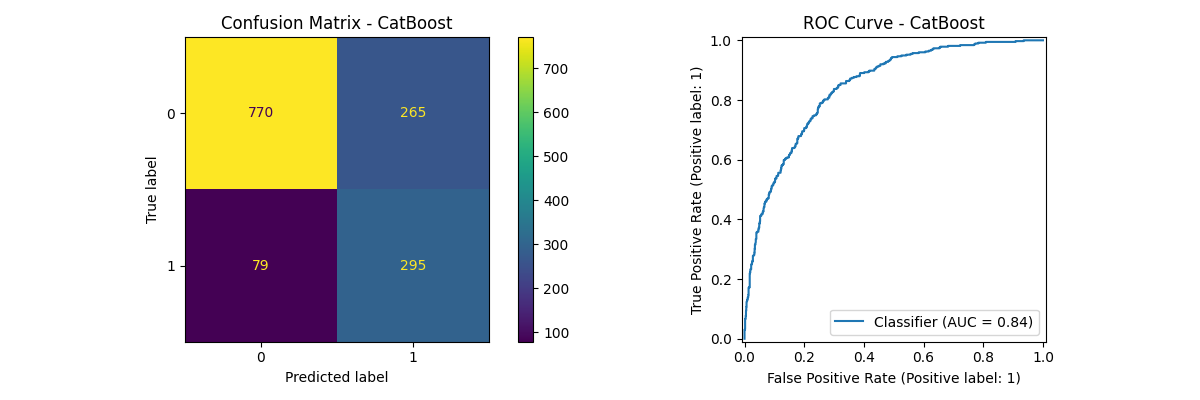
\includegraphics[width=0.95\textwidth]{models/CatBoost_eval.png}
\caption{Matrice de confusion et courbe ROC du modèle CatBoost}
\end{figure}

\subsection{Optimisation des hyperparamètres}

Une optimisation complémentaire est réalisée avec
\texttt{RandomizedSearchCV} pour XGBoost et CatBoost, et
\texttt{GridSearchCV} pour la régression logistique. La métrique optimisée est
le ROC-AUC.

La recherche aléatoire explore différentes combinaisons du nombre d'arbres, de
la profondeur, du taux d'apprentissage et des paramètres d'échantillonnage.
La validation croisée estime la stabilité des configurations sur plusieurs
sous-ensembles du jeu d'entraînement. Le jeu Test reste réservé à l'évaluation
finale.

\begin{table}[H]
\centering
\caption{Meilleurs hyperparamètres identifiés}
\begin{tabularx}{\textwidth}{p{0.22\textwidth}X}
\toprule
\textbf{Modèle} & \textbf{Configuration retenue}\\
\midrule
XGBoost &
200 arbres, profondeur 3, taux d'apprentissage 0,05, sous-échantillonnage
0,7, \texttt{colsample\_bytree}=0,7 et \texttt{min\_child\_weight}=5.\\
CatBoost &
200 itérations, profondeur 4, taux d'apprentissage 0,05 et
\texttt{l2\_leaf\_reg}=7.\\
Régression logistique &
$C=10$ avec le solveur \texttt{lbfgs}.\\
\bottomrule
\end{tabularx}
\end{table}

\begin{table}[H]
\centering
\caption{Résultats après optimisation}
\begin{tabular}{lcc}
\toprule
\textbf{Modèle} & \textbf{ROC-AUC validation croisée} &
\textbf{ROC-AUC test}\\
\midrule
XGBoost optimisé & 0,850 & \textbf{0,847}\\
CatBoost optimisé & \textbf{0,851} & 0,847\\
Régression logistique optimisée & 0,846 & 0,840\\
\bottomrule
\end{tabular}
\end{table}

L'optimisation améliore notamment le ROC-AUC test de XGBoost, qui passe de
0,828 à 0,847. Les modèles, le préprocesseur et les résultats sont sauvegardés
dans le dossier \filepath{models/} au format \texttt{.pkl}, \texttt{.csv} et
\texttt{.png}.

\subsection{Choix du modèle et limites de l'évaluation}

CatBoost est retenu comme meilleur modèle de base, car il obtient le meilleur
Recall, le meilleur F1-score et le meilleur ROC-AUC. Après optimisation,
XGBoost et CatBoost atteignent des performances très proches. Le choix de
production peut donc intégrer d'autres critères : temps d'inférence, facilité
de maintenance, stabilité des scores et coût des erreurs.

L'évaluation actuelle repose sur une séparation unique Train/Test issue d'un
dataset historique. Elle ne mesure pas encore la dérive temporelle, les
changements de comportement ou l'impact réel des actions commerciales. Une
validation sur des périodes futures serait nécessaire avant une utilisation
opérationnelle à grande échelle.

%==============================================================================
\section{Chapitre 3 : Interprétation et recommandations métier}

\subsection{Objectif de l'interprétabilité}

Un score prédictif n'est réellement utile que s'il peut être compris et relié
à une décision. L'interprétabilité permet de vérifier que le modèle s'appuie
sur des variables cohérentes, d'identifier les populations prioritaires et de
formuler des actions de fidélisation. Elle contribue également à détecter des
biais potentiels ou des dépendances excessives à certaines caractéristiques.

\subsection{Analyse de feature importance}

L'importance des variables permet de comprendre les facteurs utilisés par les
modèles. Pour XGBoost, la variable dominante est le contrat mensuel, suivie du
service Internet par fibre optique. Pour CatBoost, l'ancienneté, les charges
totales et les charges mensuelles occupent les premières positions.

\begin{figure}[H]
\centering
\begin{minipage}{0.49\textwidth}
    \centering
    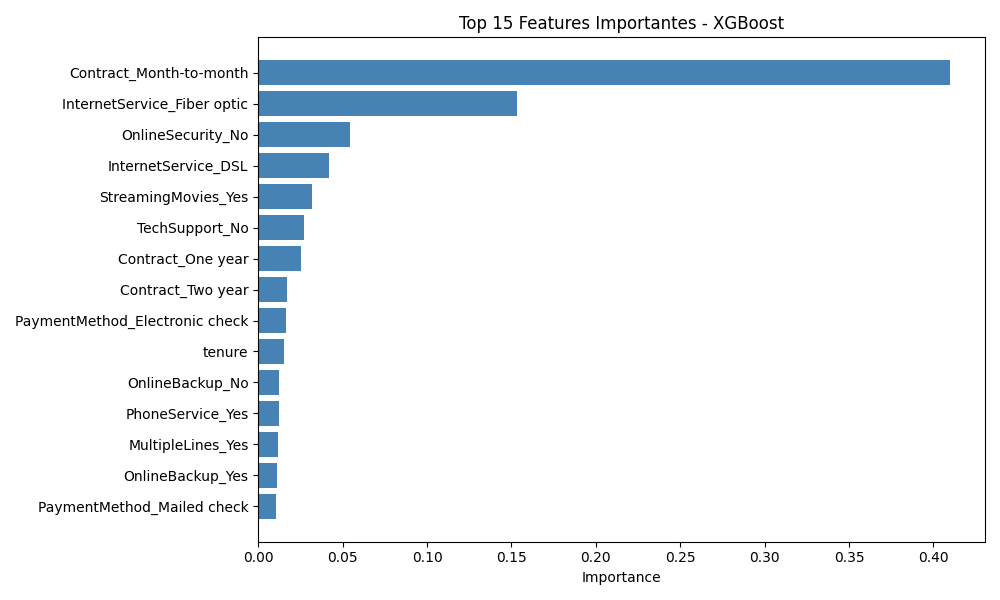
\includegraphics[width=\linewidth]{models/XGBoost_feature_importance.png}
    \caption*{XGBoost}
\end{minipage}
\hfill
\begin{minipage}{0.49\textwidth}
    \centering
    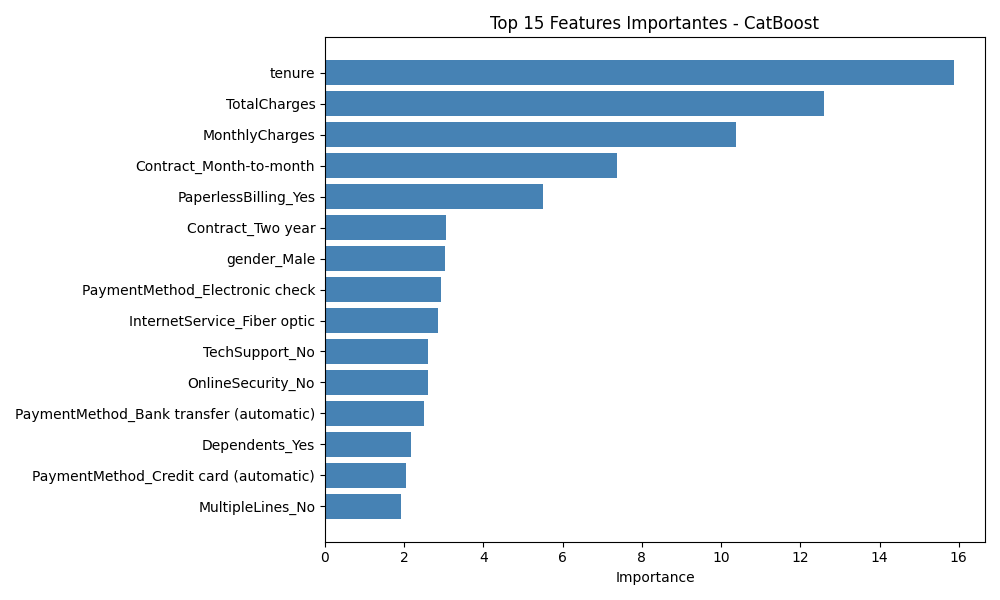
\includegraphics[width=\linewidth]{models/CatBoost_feature_importance.png}
    \caption*{CatBoost}
\end{minipage}
\caption{Variables les plus influentes selon les modèles}
\end{figure}

Les facteurs récurrents entre l'analyse exploratoire et les modèles sont :
\begin{itemize}[leftmargin=*]
    \item le contrat mensuel, fortement associé au churn ;
    \item une faible ancienneté ;
    \item des charges mensuelles et totales élevées ;
    \item la fibre optique ;
    \item l'absence de support technique ou de sécurité en ligne ;
    \item le paiement par chèque électronique.
\end{itemize}

\begin{warningbox}
La feature importance décrit l'influence d'une variable sur la prédiction, mais
ne prouve pas une relation causale. Les actions métier doivent donc être
validées par des tests contrôlés et un suivi de leur efficacité.
\end{warningbox}

\subsection{Lecture croisée des modèles}

Les importances ne sont pas directement comparables en valeur absolue entre
XGBoost, CatBoost et la régression logistique, car chaque algorithme les calcule
différemment. Leur classement permet toutefois d'identifier des facteurs
récurrents. Le contrat, l'ancienneté, les charges et le service Internet
apparaissent à la fois dans l'analyse exploratoire et dans les trois familles
de modèles.

\begin{table}[H]
\centering
\caption{Synthèse des facteurs de risque et interprétation métier}
\begin{tabularx}{\textwidth}{p{0.27\textwidth}X}
\toprule
\textbf{Facteur} & \textbf{Interprétation et piste d'action}\\
\midrule
Contrat mensuel &
Faible engagement ; proposer un avantage conditionné à un contrat annuel.\\
Faible ancienneté &
Phase d'adoption sensible ; renforcer l'accompagnement des nouveaux clients.\\
Charges élevées &
Risque de perception négative du rapport qualité-prix ; effectuer une revue
de facture ou proposer une offre adaptée.\\
Fibre optique &
Attentes potentiellement élevées ; surveiller la qualité et la satisfaction.\\
Absence de support &
Risque de frustration non résolue ; promouvoir ou offrir temporairement
l'assistance technique.\\
\bottomrule
\end{tabularx}
\end{table}

\subsection{Segmentation du risque}

Chaque probabilité produite par le modèle est transformée en un niveau de
risque directement exploitable :
\begin{itemize}[leftmargin=*]
    \item \textcolor{successgreen}{\textbf{risque faible}} : probabilité
    inférieure à 30\,\% ;
    \item \textcolor{warningorange}{\textbf{risque moyen}} : probabilité entre
    30\,\% et 60\,\% ;
    \item \textcolor{riskred}{\textbf{risque élevé}} : probabilité supérieure
    ou égale à 60\,\%.
\end{itemize}

La segmentation combine ensuite le score avec l'ancienneté, le montant des
charges et le type de contrat. Elle distingue notamment les clients à forte
valeur, les nouveaux clients vulnérables et les clients sans engagement à
convertir.

Le seuil de 60\,\% permet d'identifier les clients nécessitant une intervention
rapide, tandis que le niveau moyen sert à déclencher des actions préventives
moins coûteuses. Ces seuils constituent des règles métier initiales. Ils
devraient être optimisés à partir du coût des campagnes, de la valeur client et
du taux de succès des actions.

\subsection{Recommandations de fidélisation}

\begin{table}[H]
\centering
\caption{Recommandations automatisées par segment}
\begin{tabularx}{\textwidth}{>{\bfseries}p{0.27\textwidth}X}
\toprule
\textbf{Segment} & \textbf{Action recommandée}\\
\midrule
Forte valeur à risque &
Appel prioritaire sous 24 heures, remise personnalisée et revue de facture.\\
Nouveau client vulnérable &
Renforcer l'accueil, réaliser un appel de satisfaction et offrir une
assistance.\\
Sans engagement à convertir &
Proposer un contrat annuel avec remise et avantage de fidélité.\\
Client à surveiller &
Envoyer une enquête de satisfaction et une offre ciblée.\\
Client fidèle à valoriser &
Valoriser l'ancienneté et proposer un avantage exclusif.\\
Client stable &
Maintenir la relation standard et suivre régulièrement la satisfaction.\\
\bottomrule
\end{tabularx}
\end{table}

\subsection{Mise à disposition avec Streamlit}

L'application principale \filepath{app.py} permet de saisir le profil d'un
client, de choisir un modèle et d'obtenir :
\begin{itemize}[leftmargin=*]
    \item une prédiction Churn ou No Churn ;
    \item la probabilité estimée de churn ;
    \item le segment de risque et une recommandation personnalisée ;
    \item les métriques, courbes ROC et importances de variables.
\end{itemize}

Le dashboard \filepath{Bonus/dashboard_analytics.py} fournit une vue agrégée
avec filtres, indicateurs de churn, revenu à risque, graphiques analytiques et
table des clients à risque élevé.

\begin{infobox}
Le même préprocesseur sauvegardé lors de l'entraînement est réutilisé pour les
prédictions Streamlit. Cette cohérence garantit que les données saisies suivent
exactement les transformations apprises pendant l'entraînement.
\end{infobox}

\subsection{Parcours utilisateur et architecture de déploiement}

Dans l'application principale, l'utilisateur sélectionne un modèle et renseigne
les informations du client dans la barre latérale. Le formulaire est transformé
par le préprocesseur sauvegardé, puis transmis au modèle afin de produire une
classe et une probabilité. Le résultat est enrichi par le module de rétention
avant d'être affiché avec les métriques et les graphiques d'analyse.

Le dashboard analytique applique le même principe sur un ensemble de clients.
Il permet de filtrer le portefeuille, de calculer les scores de risque et de
suivre les indicateurs de churn. La séparation entre logique de préparation,
modélisation, prédiction et interface réduit la duplication et facilite les
évolutions futures.

\subsection{Suivi opérationnel recommandé}

Une mise en production durable nécessite un suivi régulier :
\begin{itemize}[leftmargin=*]
    \item contrôler la distribution des variables et la dérive des scores ;
    \item suivre le Recall, la Precision et le ROC-AUC sur les nouvelles
    périodes ;
    \item mesurer le taux d'acceptation et l'efficacité des recommandations ;
    \item recalibrer les seuils selon les coûts et la capacité des équipes ;
    \item réentraîner le modèle lorsque les performances se dégradent.
\end{itemize}

%==============================================================================
\clearpage
\section*{Conclusion générale}
\addcontentsline{toc}{section}{Conclusion générale}

Ce projet a permis de concevoir une solution complète de prédiction du churn
client, depuis l'analyse des données jusqu'à la mise à disposition des
résultats dans une interface interactive. Le pipeline développé assure le
nettoyage, l'imputation, l'encodage et la séparation rigoureuse des données. La
réutilisation du préprocesseur pendant l'inférence garantit la cohérence entre
l'entraînement et les prédictions réalisées dans Streamlit.

La comparaison de XGBoost, CatBoost et de la régression logistique montre que
les approches étudiées offrent une bonne capacité de classement. CatBoost
obtient les meilleurs résultats parmi les modèles de base, avec un ROC-AUC de
0,842 et un Recall de 0,789. L'optimisation des hyperparamètres améliore
notamment XGBoost jusqu'à un ROC-AUC test de 0,847. Ces résultats confirment
l'intérêt du gradient boosting pour l'analyse de données clients tabulaires.

Au-delà de la performance prédictive, l'analyse exploratoire et la feature
importance ont permis d'identifier les principaux facteurs associés au churn :
contrat mensuel, faible ancienneté, charges élevées, fibre optique et absence
de certains services d'assistance. Le système transforme ces informations en
segments de risque et en recommandations de fidélisation directement
exploitables.

La solution présente néanmoins plusieurs limites. Le dataset ne contient pas
d'historique temporel détaillé, d'informations sur les interactions avec le
service client ni de mesure du résultat des campagnes de rétention. De plus,
les importances de variables ne permettent pas d'établir une causalité. Une
validation métier reste donc indispensable avant toute automatisation des
décisions.

Les perspectives prioritaires consistent à intégrer des données plus récentes,
mettre en place une surveillance de dérive, calibrer les probabilités, optimiser
le seuil selon la valeur économique des clients et évaluer les recommandations
par des tests A/B. Une telle évolution permettrait de passer d'un prototype
prédictif à un véritable système continu d'aide à la décision.

%==============================================================================
\clearpage
\section*{Bibliographie}
\addcontentsline{toc}{section}{Bibliographie}

\begin{thebibliography}{9}

\bibitem{chen2016xgboost}
T. Chen et C. Guestrin,
\textit{XGBoost: A Scalable Tree Boosting System},
Proceedings of the 22nd ACM SIGKDD International Conference on Knowledge
Discovery and Data Mining, 2016.

\bibitem{prokhorenkova2018catboost}
L. Prokhorenkova, G. Gusev, A. Vorobev, A. V. Dorogush et A. Gulin,
\textit{CatBoost: Unbiased Boosting with Categorical Features},
Advances in Neural Information Processing Systems, 2018.

\bibitem{pedregosa2011sklearn}
F. Pedregosa et al.,
\textit{Scikit-learn: Machine Learning in Python},
Journal of Machine Learning Research, vol. 12, pp. 2825--2830, 2011.

\bibitem{fawcett2006roc}
T. Fawcett,
\textit{An Introduction to ROC Analysis},
Pattern Recognition Letters, vol. 27, no. 8, pp. 861--874, 2006.

\bibitem{streamlitdocs}
Streamlit,
\textit{Streamlit Documentation},
\url{https://docs.streamlit.io/}, consulté en juin 2026.

\bibitem{xgboostdocs}
XGBoost Developers,
\textit{XGBoost Documentation},
\url{https://xgboost.readthedocs.io/}, consulté en juin 2026.

\bibitem{catboostdocs}
CatBoost Developers,
\textit{CatBoost Documentation},
\url{https://catboost.ai/}, consulté en juin 2026.

\end{thebibliography}

%==============================================================================
\clearpage
\section{Annexes}

\subsection{Structure du repository}

\begin{verbatim}
churn_project/
|-- data/                 Dataset CSV
|-- notebooks/            EDA et expérimentations
|-- src/                  Prétraitement, entraînement et prédiction
|-- models/               Modèles et résultats sauvegardés
|-- Bonus/                Dashboard, API et optimisation
|-- tests/                Tests automatisés
|-- app.py                Application Streamlit
|-- train_and_evaluate.py Pipeline d'entraînement
`-- requirements.txt      Dépendances Python
\end{verbatim}

\subsection{Commandes d'exécution}

\begin{verbatim}
python -m pip install -r requirements.txt
python train_and_evaluate.py
python Bonus/hyperparameter_tuning.py --quick
python -m streamlit run app.py
python -m streamlit run Bonus/dashboard_analytics.py
python -m pytest -q
\end{verbatim}

\end{document}
